\documentclass[xetex,mathserif,serif]{beamer}

\usepackage{xunicode}
\usepackage{xltxtra}
\usepackage{color}
\usepackage{url}
\usepackage{listings}
\usepackage{fontspec}
\usepackage{geometry}
\usepackage{lastpage}
\usepackage{fancyhdr}
\usepackage{amsmath}
\usepackage{amsthm}
\usepackage{amssymb}
\usepackage{blkarray}
\usepackage{multicol}
\usepackage{relsize}

\definecolor{solarized@base03}{HTML}{002B36}
\definecolor{solarized@base02}{HTML}{073642}
\definecolor{solarized@base01}{HTML}{586e75}
\definecolor{solarized@base00}{HTML}{657b83}
\definecolor{solarized@base0}{HTML}{839496}
\definecolor{solarized@base1}{HTML}{93a1a1}
\definecolor{solarized@base2}{HTML}{EEE8D5}
\definecolor{solarized@base3}{HTML}{FDF6E3}
\definecolor{solarized@yellow}{HTML}{B58900}
\definecolor{solarized@orange}{HTML}{CB4B16}
\definecolor{solarized@red}{HTML}{DC322F}
\definecolor{solarized@magenta}{HTML}{D33682}
\definecolor{solarized@violet}{HTML}{6C71C4}
\definecolor{solarized@blue}{HTML}{268BD2}
\definecolor{solarized@cyan}{HTML}{2AA198}
\definecolor{solarized@green}{HTML}{859900}
\definecolor{yaleblue}{HTML}{0E4C92}

\newcommand{\yellow}[1]{\textcolor{solarized@yellow}{#1}}
\newcommand{\orange}[1]{\textcolor{solarized@orange}{#1}}
\newcommand{\red}[1]{\textcolor{solarized@red}{#1}}
\newcommand{\magenta}[1]{\textcolor{solarized@magenta}{#1}}
\newcommand{\violet}[1]{\textcolor{solarized@violet}{#1}}
\newcommand{\blue}[1]{\textcolor{solarized@blue}{#1}}
\newcommand{\cyan}[1]{\textcolor{solarized@cyan}{#1}}
\newcommand{\green}[1]{\textcolor{solarized@green}{#1}}
\newcommand{\yblue}[1]{\textcolor{yaleblue}{#1}}

\setbeamertemplate{navigation symbols}{}
% \setbeamerfont{title}{family=\old}
% \setbeamerfont{author}{family=\tfont}%
% \setbeamerfont{frametitle}{family=\oldA}
% \setbeamerfont{date}{family=\dfont}

% \addtobeamertemplate{navigation symbols}{}{%
%     \usebeamerfont{footline}%
%     \usebeamercolor[fg]{footline}%
%     \hspace{1em}%
%     \insertframenumber/\inserttotalframenumber
% }

\setbeamertemplate{footline}[text line]{%
  \parbox{0.99\linewidth}{
    \normalsize\vspace*{-24pt}\hfill{\color{solarized@base00}\insertframenumber/\inserttotalframenumber}
  }
}


\setbeamertemplate{itemize items}{--}
\setbeamercolor*{item}{fg=black}

\defaultfontfeatures{Mapping=tex-text}
\hypersetup{pdfstartview={FitH}}

\newcommand{\old}[1]{\fontspec[Alternate=1,Ligatures={Common}]{Hoefler Text}\fontsize{18pt}{30pt}\selectfont #1}%
\newcommand{\oldA}[1]{\fontspec[Alternate=1,Ligatures={Common, Rare}]{Hoefler Text}\fontsize{12pt}{15pt}\selectfont #1}%
\newcommand{\oldB}[1]{\fontspec[Ligatures={Common}]{Didot}\fontsize{12pt}{15pt}\color{solarized@base02}\selectfont #1}%
\newcommand{\tfont}[1]{\fontspec[Alternate=1,Ligatures={Common}]{Hoefler Text}\fontsize{12pt}{20pt}\selectfont #1}%
\newcommand{\dfont}[1]{\fontspec[Ligatures={Common}]{Didot}\fontsize{12pt}{12pt}\selectfont #1}%

% \newcommand{\minimize}{\mathop{\mathrm{minimize}}}
\newcommand{\argmin}{\mathop{\mathrm{arg\,min}}}
\newcommand{\argmax}{\mathop{\mathrm{arg\,max}}}
\newcommand{\st}{\mathop{\mathrm{subject\,\,to}}}

\newcommand\independent{\protect\mathpalette{\protect\independenT}{\perp}}
\def\independenT#1#2{\mathrel{\rlap{$#1#2$}\mkern2mu{#1#2}}}

\setlength{\parindent}{0pt}
\setlength{\parskip}{12pt}

\setromanfont [Ligatures={Common}, Numbers={OldStyle}, Variant=01,
 BoldFont={LinLibertine_RB.otf},
 ItalicFont={LinLibertine_RI.otf},
 BoldItalicFont={LinLibertine_RBI.otf}
 ]{LinLibertine_R.otf}



\newcommand{\blueone}{{\color{yaleblue} 1}}
\newcommand{\greyzero}{{\color{solarized@base00} 0}}
\usepackage{sty/personalmacros}
\usepackage{sty/personalslides}

\begin{document}
%%%%%%%%%%%%%%%%%%%%%%%%%%%%%%%%%%%%%%%%%%%%%%%%%%%%%%%%%%%%%%%%%%%%%%%%%%%%%%%
% Manifest
% --------
% - Title
% - Outline
% - Review of Graphical Models
% - Review of Multivariate Gaussian
% - Precision Matrices in Context of Gaussian Graphical Models
% - Pairwise Inference for Entrywise Recovery
% - Upper Bound ($\ell_infty$ norm)
%   - Statement of Theorems 2 and 3
%   - Proof / Intuition for Theorems 2 and 3
% - Lower Bound ($\ell_infty$ norm)
%   - Statement of Theorem 5
%   - Proof / Intuition for Theorem 5
% - Next Steps
%%%%%%%%%%%%%%%%%%%%%%%%%%%%%%%%%%%%%%%%%%%%%%%%%%%%%%%%%%%%%%%%%%%%%%%%%%%%%%%
\begin{frame}[fragile] \frametitle{}
\vfill
\vspace{0.2cm}
{
    \color{yaleblue}
    \fontsize{0.5cm}{0cm}\selectfont
    Midterm Presentation: \\
}
\vspace{1.0cm}
{
    \fontsize{0.7cm}{0cm}\selectfont
    Risk Properties in Sparse Precision Matrix Estimation\\
}

\hfill

\vspace{1.8cm}
\begin{minipage}{1.0\textwidth}\raggedleft
    \color{yaleblue}
    Addison J. Hu   \\
    Statistics 490 \\
    01 March 2017
\end{minipage}
\end{frame}
%%%%%%%%%%%%%%%%%%%%%%%%%%%%%%%%%%%%%%%%%%%%%%%%%%%%%%%%%%%%%%%%%%%%%%%%%%%%%%%
% Outline
%%%%%%%%%%%%%%%%%%%%%%%%%%%%%%%%%%%%%%%%%%%%%%%%%%%%%%%%%%%%%%%%%%%%%%%%%%%%%%%
\begin{frame}[fragile] \frametitle{}
    \slideheader{Outline}
    \begin{enumerate}
        \item Graphical Models \& Multivariate Gaussian
        \item Pairwise Inference for Entrywise Recovery of $\Sigma^{-1}$
        \item Risk Bounds
        \item Banded Case
    \end{enumerate}
\end{frame}
%%%%%%%%%%%%%%%%%%%%%%%%%%%%%%%%%%%%%%%%%%%%%%%%%%%%%%%%%%%%%%%%%%%%%%%%%%%%%%%
% Refresher
%%%%%%%%%%%%%%%%%%%%%%%%%%%%%%%%%%%%%%%%%%%%%%%%%%%%%%%%%%%%%%%%%%%%%%%%%%%%%%%
\begin{frame}[fragile] \frametitle{}
    \sectionslide{Background}
\end{frame}
%%%%%%%%%%%%%%%%%%%%%%%%%%%%%%%%%%%%%%%%%%%%%%%%%%%%%%%%%%%%%%%%%%%%%%%%%%%%%%%
\begin{frame}[fragile] \frametitle{}
    \slideheader{Graphical Models}
    \begin{itemize}
        \item Graphical models provide a framework within which to consider
            dependence structure within a group of variables.
        \item In doing so, we may relax the i.i.d. assumption and still perform
            inference feasibly.
        \item Examples:
            \begin{itemize}
                \item Facebook users graph
                \item Gene interaction networks
            \end{itemize}
    \end{itemize}
\end{frame}
%%%%%%%%%%%%%%%%%%%%%%%%%%%%%%%%%%%%%%%%%%%%%%%%%%%%%%%%%%%%%%%%%%%%%%%%%%%%%%%
\begin{frame}[fragile] \frametitle{}
    \slideheader{Markov Random Fields}
    \begin{itemize}
        \item Consider a graph $G = (V, E)$, and a corresponding set of
            random variables $\{X_i\}_{i=1}^{|V|}$, where the random variables
            are indexed by $u \in V$.
        \item \textbf{Pairwise Markov property:} $X_u \indep X_v | X_{V
            \setminus\{u, v\}}$ for any two non-adjacency nodes $u, v$.
        \item \textbf{Local Markov property:} $X_u \indep X_{V \setminus
            \mathrm{cl}(u)} | X_{\mathrm{nb}(u)}$ for any node $v$.
        \item \textbf{Global Markov property:} $X_A \indep X_B | X_S$ for
            disjoint $A, B \subset V$, and a separating subset $S$.
        \item Inference is easy when the edges are known; but is more
            interesting when they are unknown.
    \end{itemize}
    % https://en.wikipedia.org/wiki/Markov_random_field
\end{frame}
%%%%%%%%%%%%%%%%%%%%%%%%%%%%%%%%%%%%%%%%%%%%%%%%%%%%%%%%%%%%%%%%%%%%%%%%%%%%%%%
\begin{frame}[fragile] \frametitle{}
    \slideheader{Example: Hub and Spoke Model}
    \vspace{1cm}
    \begin{columns}[T]
        \begin{column}{.48\textwidth}
            $$
            \bmat{
                \blueone & \greyzero & \greyzero & \blueone & \greyzero &
                \greyzero & \greyzero   \\ 
                \greyzero & \blueone & \greyzero & \blueone & \greyzero &
                \greyzero & \greyzero   \\ 
                \greyzero & \greyzero & \blueone & \blueone & \greyzero &
                \greyzero & \greyzero   \\ 
                \blueone & \blueone & \blueone & \blueone & \blueone & \blueone
                & \blueone   \\ 
                \greyzero & \greyzero & \greyzero & \blueone & \blueone &
                \greyzero & \greyzero   \\ 
                \greyzero & \greyzero & \greyzero & \blueone & \greyzero &
                \blueone & \greyzero   \\ 
                \greyzero & \greyzero & \greyzero & \blueone & \greyzero &
                \greyzero & \blueone
            }
            $$
        \end{column}
        \hfill
        \begin{column}{.48\textwidth}
            \vspace{-0.2cm}
            \hspace{-0.5cm}
            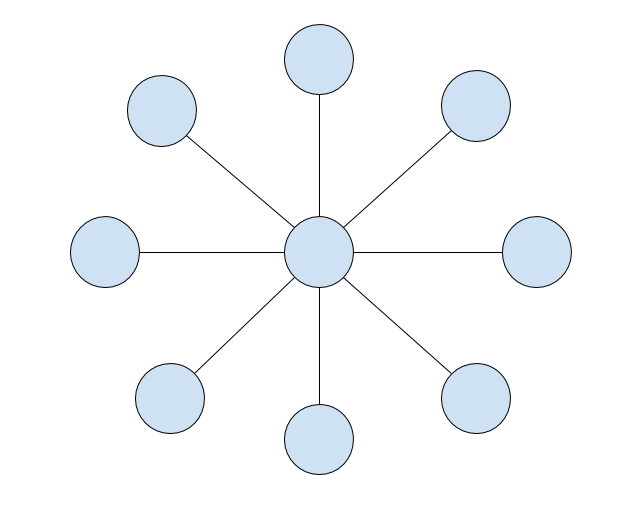
\includegraphics[scale=0.25]{img/spokes.png}
        \end{column}
    \end{columns}
\end{frame}
%%%%%%%%%%%%%%%%%%%%%%%%%%%%%%%%%%%%%%%%%%%%%%%%%%%%%%%%%%%%%%%%%%%%%%%%%%%%%%%
\begin{frame}[fragile] \frametitle{}
    \slideheader{Multivariate Gaussian}

    Suppose $X \dist \Nn(\mu, \Sigma)$. Its density function is given by:
	$$
    p(\xx) = \left(2\pi\right)^{-\frac{p}{2}}\left|\Sigma\right|^{-\frac{1}{2}}
    \exp\lc-\frac{1}{2}(\xx - \mathbf{\mu})^\top \Sigma^{-1}
    (\xx - \mathbf{\mu})\rc
    $$
    \vspace{-0.7cm}
    \begin{itemize}
        \item Closure properties:
            \begin{itemize}
                \item Sum of independent Gaussian random variables is Gaussian.
                \item Marginal of a joint Gaussian distribution is Gaussian.
                \item Condition of a joint Gaussian distribution is Gaussian.
            \end{itemize}
        \item The sparsity pattern of $\Sigma^{-1}$ concides with the adjacency
            matrix of the associated MRF.
    \end{itemize}
    % http://cs229.stanford.edu/section/more_on_gaussians.pdf
\end{frame}
%%%%%%%%%%%%%%%%%%%%%%%%%%%%%%%%%%%%%%%%%%%%%%%%%%%%%%%%%%%%%%%%%%%%%%%%%%%%%%%
\begin{frame}[fragile] \frametitle{}
    \slideheader{Multivariate Gaussian, cont.}

	\begin{itemize}
        \item Closure under marginalization:  Suppose $A \subset V$.  Then
            $$
            \Sigma_{A} = \lp\Sigma_{ij}\rp_{i\in A, j \in A}
            $$
        \item Closure under conditioning: Suppose  $A, B \subset V$, $A \cup B
            = V, A \cap B = \varnothing$.  Then:
            \begin{align*}
                \lp \Omega_A \rp ^{-1}  &= \Sigma_{A|B}   \\
                \lp \Sigma_A \rp ^{-1}  &= \Omega_{A|B}   \\
            \end{align*}
	\end{itemize}
\end{frame}
%%%%%%%%%%%%%%%%%%%%%%%%%%%%%%%%%%%%%%%%%%%%%%%%%%%%%%%%%%%%%%%%%%%%%%%%%%%%%%%
% Pairwise Recovery
%%%%%%%%%%%%%%%%%%%%%%%%%%%%%%%%%%%%%%%%%%%%%%%%%%%%%%%%%%%%%%%%%%%%%%%%%%%%%%%
\begin{frame}[fragile] \frametitle{}
    \sectionslide{Precision Matrix Estimation}
\end{frame}
%%%%%%%%%%%%%%%%%%%%%%%%%%%%%%%%%%%%%%%%%%%%%%%%%%%%%%%%%%%%%%%%%%%%%%%%%%%%%%%
\begin{frame}[fragile] \frametitle{}
    \slideheader{Maximum Likelihood Estimation}
    \vspace{0.5cm}

    Assume $\mu = 0$.  Then the maximum likelihood estimation problem is:
	\begin{align*}
		\maximize{
            \log\det|\Sigma^{-1}| - \langle \hat\Sigma, \Sigma^{-1} \rangle
		}{\Sigma}{\Sigma \gengeq 0}
	\end{align*}
    \vspace{-0.8cm}
    \begin{itemize}
        \item Maximum Likelihood Estimate given by $\hat\Sigma = 
            \frac{1}{n} \XX^\top \XX$.
        \item Idea: $\hat\Omega = \hat\Sigma^{-1}$.
        \item Issues:
            \begin{itemize}
                \item Invertibility \& Conditioning
                \item Noise \& Sparsity
            \end{itemize}
    \end{itemize}
\end{frame}
%%%%%%%%%%%%%%%%%%%%%%%%%%%%%%%%%%%%%%%%%%%%%%%%%%%%%%%%%%%%%%%%%%%%%%%%%%%%%%%
\begin{frame}[fragile] \frametitle{}
    \slideheader{Graphical Lasso}

    \vspace{0.6cm}
    To encourage sparsity, Tibshirani \textit{et al} proposed imposing an
    entrywise $\ell_1$ penalty on $\Omega$.

    \begin{align*}
        \maximize{
            \log\det|\Omega| - \langle \hat\Sigma, \Omega \rangle
            - \rho \norm{\Omega}_1
        }{\Omega}{\Omega \gengeq 0}
    \end{align*}
\end{frame}
%%%%%%%%%%%%%%%%%%%%%%%%%%%%%%%%%%%%%%%%%%%%%%%%%%%%%%%%%%%%%%%%%%%%%%%%%%%%%%%
\begin{frame}[fragile] \frametitle{}
    \slideheader{Asymptotic Normal Thresholding (ANT)}
    \begin{itemize}
        \item Goal: Obtain entrywise estimates $\hat\omega_{ij}$ of $\Omega$
            that are asymptotically norm and minimax, and then threshold to
            enforce sparsity.
        \item Idea: For each pair $A = \{i, j\}$, regress the variables $X_i,
            X_j$ on all other variables:
            $$
            \XX_A = \XX_{A^c}\beta + \epsilon_A
            $$
            where $\epsilon_A$ is a noise term, distributed normally with mean
            zero, and which are independent of $\XX_{A^c}$.
        \item Rationale: $\Omega_{A, A}^{-1} \defas \Theta_{A, A} \defas
            \Sigma_{A|A^c} = \var(X_A|X_{A^c}) = \var(\epsilon_A)$.  Errors
            give entries of precision matrix.
    \end{itemize}
\end{frame}
%%%%%%%%%%%%%%%%%%%%%%%%%%%%%%%%%%%%%%%%%%%%%%%%%%%%%%%%%%%%%%%%%%%%%%%%%%%%%%%
\begin{frame}[fragile] \frametitle{}
    \slideheader{Oracle MLE}

    \begin{itemize}
        \item Suppose we could draw from the distribution of $\epsilon_A$
            directly.  How would we estimate $\Omega_{A, A}$?  
        \item The maximum likelihood estimator in this case is:
            $$
            \Theta^{ora}_{A, A} = (\theta^{ora}_{kl})_{k, l \in A}
            = \frac{\epsilon_A^\top\epsilon_A}{n}
            $$
            where we call $\Theta^{ora}$ the \textit{oracle} MLE covariance estimates.
        \item The corresponding oracle MLE precision estimates are then given
            by:
            $$
            \Omega^{ora}_{A, A} = (\omega^{ora}_{kl})_{k, l \in A}
                = \left(\Theta^{ora}_{A, A}\right)^{-1}
            $$
    \end{itemize}
\end{frame}
%%%%%%%%%%%%%%%%%%%%%%%%%%%%%%%%%%%%%%%%%%%%%%%%%%%%%%%%%%%%%%%%%%%%%%%%%%%%%%%
\begin{frame}[fragile] \frametitle{}
    \slideheader{Residual Estimates}
    \begin{itemize}
        \item In practice, we only observe $\XX$, so we must estimate
            $\epsilon_A$.
        \item Suppose we have an adequate estimates of the regression weights
            $\hat\beta$.  Then:
            $$
            \hat\epsilon_A = \XX_A - \XX_{A^c}\hat\beta
            $$
        \item Consequently:
            \vspace{-0.1cm}
            \begin{align*}
                \hat\Theta_{A, A}
                &= \frac{\hat\epsilon_A^\top\hat\epsilon_A}{n}    \\
                \hat\Omega_{A, A} &= \hat\Theta_{A, A}^{-1}
            \end{align*}
    \end{itemize}
\end{frame}
%%%%%%%%%%%%%%%%%%%%%%%%%%%%%%%%%%%%%%%%%%%%%%%%%%%%%%%%%%%%%%%%%%%%%%%%%%%%%%%
\begin{frame}[fragile] \frametitle{}
	\slideheader{Scaled Lasso Estimator}

    For each $m \in A = \{i, j\}$, perform the optimization: 

    $$
    \left\{\hat\beta_m, \hat\theta^{1/2}_{mm}\right\}
    =
    \arg\min_{\substack{b\in\RR^{p-2},\\\sigma \in \RR^+}}
    \left\{
    \frac{\norm{\XX_m - \XX_{A^c}b}^2}{2n\sigma}
    + \frac{\sigma}{2} 
    + \lambda\sum_{k\in A^c}\frac{\norm{\XX_k}}{\sqrt{n}}|b_k|
    \right\}
    $$
    
    Intuitively, the scaling factor on the $\ell_1$ penalty implicitly standardizes
    the design vector to length $\sqrt{n}$ such that the $\ell_1$ penalty is
    applied to the new coefficients $\frac{\norm{\XX_k}}{\sqrt n}b_k$.

\end{frame}
%%%%%%%%%%%%%%%%%%%%%%%%%%%%%%%%%%%%%%%%%%%%%%%%%%%%%%%%%%%%%%%%%%%%%%%%%%%%%%%
% Risk Bounds
%%%%%%%%%%%%%%%%%%%%%%%%%%%%%%%%%%%%%%%%%%%%%%%%%%%%%%%%%%%%%%%%%%%%%%%%%%%%%%%
\begin{frame}[fragile] \frametitle{}
    \sectionslide{Risk Bounds}
\end{frame}
%%%%%%%%%%%%%%%%%%%%%%%%%%%%%%%%%%%%%%%%%%%%%%%%%%%%%%%%%%%%%%%%%%%%%%%%%%%%%%%
\begin{frame}[fragile] \frametitle{}
    \slideheader{Minimaxity}

    \vspace{0.5cm}
    Recall that we call an estimator $\delta^*$ \textit{minimax} if it achieves
    the minimax risk:
    $$
    \sup_{\theta\in\Theta} R(\delta^*, \theta)
    =  \inf_\delta \sup_{\theta\in\Theta} R(\delta, \theta)
    \defas \text{minimax risk}
    $$
    where $R(\delta, \theta)$ is a risk function:
    $$
    R(\delta, \theta) \defas \EE_{X|\theta}\; \ell(\delta(X), \theta)
    $$
\end{frame}
%%%%%%%%%%%%%%%%%%%%%%%%%%%%%%%%%%%%%%%%%%%%%%%%%%%%%%%%%%%%%%%%%%%%%%%%%%%%%%%
\begin{frame}[fragile] \frametitle{}
    \slideheader{Parameter Space Construction}
    \vspace{0.5cm}

    We consider the following parameter space for $\lambda > 0$:
    $$
    \mathcal{G}^* = \left\{
    \Omega: s_\lambda(\Omega) \leq s, M^{-1}
        \leq \lambda_\mathrm{min}(\Omega)
        \leq \lambda_\mathrm{max}(\Omega)
        \leq M
    \right\}
    $$
    where
    $$
    s_\lambda = s_\lambda(\Omega) = \max_j\sum_{i\neq j}
    \min\left\{1, \frac{|\omega_{ij}|}{\lambda}\right\}
    $$
    for $\Omega = (\omega_{ij})_{1\leq i, j\leq p}$.

    The authors take $\lambda$ on the order $\sqrt\frac{\log p}{n}$ in this
    paper.
    %% TODO: Why?

\end{frame}
%%%%%%%%%%%%%%%%%%%%%%%%%%%%%%%%%%%%%%%%%%%%%%%%%%%%%%%%%%%%%%%%%%%%%%%%%%%%%%%
\begin{frame}[fragile] \frametitle{}
    \slideheader{Risk Upper Bound}

    \begin{itemize}
        \item A risk upper bound on an estimator gives a guarantee on its
            worst case performance.
        \item The ANT estimator achieves, for some constants $C_2, C_3$,
            the following bounds in probability:
            \begin{align*}
                \hspace{-0.8cm}
            \max_{\Omega\in\Gg^*(M, s, \lambda)}\max_{1 \leq i \leq j \leq p}
            \PP\left\{
            |\hat\omega_{ij} - \omega_{ij}| > C_2 \max\left\{
            s\frac{\log p}{n}, \sqrt\frac{1}{n}
            \right\}
            \right\} \leq \varepsilon_0
            \end{align*}
            \begin{align*}
                \hspace{-0.8cm}
            \max_{\Omega\in\Gg^*(M, s, \lambda)}
            \PP\left\{
            \norm{\hat\Omega - \Omega}_\infty > C_3 \max\left\{
            s\frac{\log p}{n}, \sqrt\frac{\log p}{n}
            \right\}
            \right\} = o(p^{-\delta + 3})
            \end{align*}
    \end{itemize}
\end{frame}
%%%%%%%%%%%%%%%%%%%%%%%%%%%%%%%%%%%%%%%%%%%%%%%%%%%%%%%%%%%%%%%%%%%%%%%%%%%%%%%
\begin{frame}[fragile] \frametitle{}
    \slideheader{Risk Upper Bound: Oracle Inequalities}

    First, we bound the distance from the estimator to the oracle MLEs.  There
    exist constants $C_1, C_1'$ such that:
    \begin{align*}
        \max_{A:A=\{i, j\}}
        \PP\left\{
        \norm{\hat\Theta_{A, A} - \Theta_{A, A}^{ora}}_\infty
        > C_1 s \frac{\log p}{n}
        \right\}\leq o(p^{-\delta + 1})
    \end{align*}
    and
    \begin{align*}
        \max_{A:A=\{i, j\}}
        \PP\left\{
        \norm{\hat\Omega_{A, A} - \Omega_{A, A}^{ora}}_\infty
        > C_1' s \frac{\log p}{n}
        \right\}\leq o(p^{-\delta + 1})
    \end{align*}
\end{frame}
%%%%%%%%%%%%%%%%%%%%%%%%%%%%%%%%%%%%%%%%%%%%%%%%%%%%%%%%%%%%%%%%%%%%%%%%%%%%%%%
\begin{frame}[fragile] \frametitle{}
    \slideheader{Risk Upper Bound: Coupling Argument}

    \begin{itemize}
        \item Denote $\kappa_{ij} = \sqrt{n}\frac{
                \omega_{ij}^{ora} - \omega_{ij}
            }{
                \sqrt{\omega_{ii}\omega_{jj} + \omega_{ij}^2}
            }$.
        \item Under suitable conditions (KMT Inequality), $\kappa_{ij}$ behaves
            roughly like a standard normal random variable.
        \item This gives a bound in probability on the deviation of
            $\omega_{ij}^{ora}$ from the true $\omega_{ij}$:
            $$
                \PP\left\{
                |\omega_{ij}^{ora} - \omega_{ij}|
                > C_4 \sqrt{\frac{1}{n}}
                \right\}
                \leq \frac{3}{4}\epsilon
            $$
        \item A similar argument gives:
            $$
                \PP\left\{
                    \norm{\hat\Omega_{A, A} - \Omega_{A, A}}_\infty
                > C_5 \sqrt{\frac{\log p}{n}}
                \right\}
                = o(p^{-\delta})
            $$
    \end{itemize}
\end{frame}
%%%%%%%%%%%%%%%%%%%%%%%%%%%%%%%%%%%%%%%%%%%%%%%%%%%%%%%%%%%%%%%%%%%%%%%%%%%%%%%
\begin{frame}[fragile] \frametitle{}
    \slideheader{Risk Lower Bound}

    \vspace{0.5cm}
    Suppose $\{X^{(i)}\}_{i=1}^n \iid \Nn(0, \Omega)$, $\Omega \in \Gg_0(M,
    k_{n, p})$.  An application of Le Cam's method yields the following minimax
    lower bounds:
    \vspace{0.2cm}
    $$
    \hspace{-0.5cm}
    \inf_{\hat\omega_{ij}} \sup_{\Gg(M, k_{n, p})}
    \PP\left\{
    |\hat\omega_{ij} - \omega_{ij}| > \max\left\{
    C_1\frac{k_{n, p}\log p}{n}, C_2 \sqrt\frac{1}{n}
    \right\}
    \right\} > c_1 > 0
    $$
    $$
    \hspace{-0.2cm}
    \inf_{\hat\Omega} \sup_{\Gg(M, k_{n, p})}
    \PP\left\{
        \norm{\hat\Omega - \Omega}_\infty > \max\left\{
    C_1'\frac{k_{n, p}\log p}{n}, C_2' \sqrt\frac{\log}{n}
    \right\}
    \right\} > c_2 > 0
    $$
    
\end{frame}
%%%%%%%%%%%%%%%%%%%%%%%%%%%%%%%%%%%%%%%%%%%%%%%%%%%%%%%%%%%%%%%%%%%%%%%%%%%%%%%
\begin{frame}[fragile] \frametitle{}
    \slideheader{Le Cam's Two-Point Argument}
    \begin{enumerate}
        \item Insight: Maximum of set bounded below by (weighted) average.
        \item Method: Construct a subparameter space $\Omega_L \in \Gg$, find
            the average risk over subparameter space.
    \end{enumerate}
    \vspace{-0.3cm}
    Example: Suppose probability distributions $P_1, P_2$ parameterized by
    $\theta_1, \theta_2$, respectively.
    \vspace{-0.2cm}
    \begin{align*}
        \sup_{\theta \in \Theta} \EE_{X|\theta} (\delta(X) - \theta)^2
        &\geq \frac{1}{2}\lb
        \EE_{X|\theta_1} (\delta(X) - \theta_1)^2
        +
        \EE_{X|\theta_2} (\delta(X) - \theta_2)^2
        \rb \\
        &=      \cdots  \\
        &\geq (\theta_1 - \theta_2)^2 \int \min\{p_1, p_2\} \dd \mu(x)
    \end{align*}
    Balancing act between maximizing $d(\theta_1, \theta_2)$ versus
    $\norm{P_1 \wedge P_2}$.
\end{frame}
%%%%%%%%%%%%%%%%%%%%%%%%%%%%%%%%%%%%%%%%%%%%%%%%%%%%%%%%%%%%%%%%%%%%%%%%%%%%%%%
\begin{frame}[fragile] \frametitle{}
    \slideheader{Risk Bounds in Matrix Norm}
    \begin{itemize}
        \item Bounds in $\norm{\cdot}_\infty$ can be turned into bounds
            in operator norm.
        \item The ANT estimator thresholds:
            $$\hat\omega_{ij}^\mathrm{thr} =
            \hat\omega_{ij}\one\lc|\omega_{ij}| >
            \sqrt{8\varepsilon(\omega_{ii} \omega_{jj} +
            \omega_{ij}^2)n^{-1}\log p}\rc$$
        \item The thresholded estimator achieves:
            $$
            \sup_{\Gg^*(M, k_{n, p}, \lambda)}
            \EE\norm{\hat\Omega_\mathrm{thr} - \Omega}^2_w \leq
            Cs^2\frac{\log p}{n}
            $$
            which is shown to be optimal in Cai, Liu, Zhou (2012).
    \end{itemize}
\end{frame}
%%%%%%%%%%%%%%%%%%%%%%%%%%%%%%%%%%%%%%%%%%%%%%%%%%%%%%%%%%%%%%%%%%%%%%%%%%%%%%%
\begin{frame}[fragile] \frametitle{}
    \sectionslide{Banded Case}
\end{frame}
%%%%%%%%%%%%%%%%%%%%%%%%%%%%%%%%%%%%%%%%%%%%%%%%%%%%%%%%%%%%%%%%%%%%%%%%%%%%%%%
\begin{frame}[fragile] \frametitle{}
    \slideheader{Banded Precision Matrix Case}
    \begin{itemize}
        \item The ANT estimator considers the general case of sparse precision
            matrices.
        \item Zhou et al (2016) introduces the ANT technique in a cosmological
            setting.
        \item OLS for entrywise estimates with assumed sparsity pattern.
        \item Off-diagonals are smoothed (assume that nearby entries are
            similar).
        \item Smoothed matrix is projected in maximum-likelihood to the space
            of symmetric positive-definite matrices.
        \item Off-diagonal thresholded to zero if maximum value fails to exceed
            some false-discovery threshold.
    \end{itemize}
\end{frame}
%%%%%%%%%%%%%%%%%%%%%%%%%%%%%%%%%%%%%%%%%%%%%%%%%%%%%%%%%%%%%%%%%%%%%%%%%%%%%%%
\begin{frame}[fragile] \frametitle{}
    \slideheader{Next Steps}
    \begin{itemize}
        \item Distill estimation technique from cosmology paper for analysis.
        \item Define a parameter space for banded precision matrices that lends
            itself to analysis.
        \item Intuition for an upper bound on risk for such an estimator,
            and proof.
        \item Identify subparameter space for lower bound, and proof.
    \end{itemize}
\end{frame}
%%%%%%%%%%%%%%%%%%%%%%%%%%%%%%%%%%%%%%%%%%%%%%%%%%%%%%%%%%%%%%%%%%%%%%%%%%%%%%%
\end{document}
